\chapter{Theory}
%\label{chap:theory} this doesn't seem to work

Theory relevant to the spectroscopy and detection of single Ba/Ba\textsuperscript{+} in SXe matrices is discussed.  

\section{Ba/Ba\textsuperscript{+} Spectroscopy in Vacuum}

The lowest-lying energy levels in vacuum for Ba and Ba\textsuperscript{+} are shown in Fig. \ref{fig:elevs}.  For Ba, the main transition is between the ground $6s^{2}$ $^{1}$S$_{0}$ to the excited $6s6p$ $^{1}$P$_{1}$ state.  Spin{\color{red}(?)}-suppressed transitions between the P state and three metastable D states results in a decay in to a D state after about 350 excitations.  For Ba\textsuperscript{+}, two strong transitions exist between the ground $6s$ $^{2}$S$_{1/2}$ \textbf{{\color{red}is the doublet correct??}} and the $6p$ $^{2}$P$_{1/2}$ and $6p$ $^{2}$P$_{3/2}$ excited states.  Transitions to the two metastable D states are higher than for the atom, resulting in a decay into a D state after about 4 excitations.

\begin{figure}[H]
	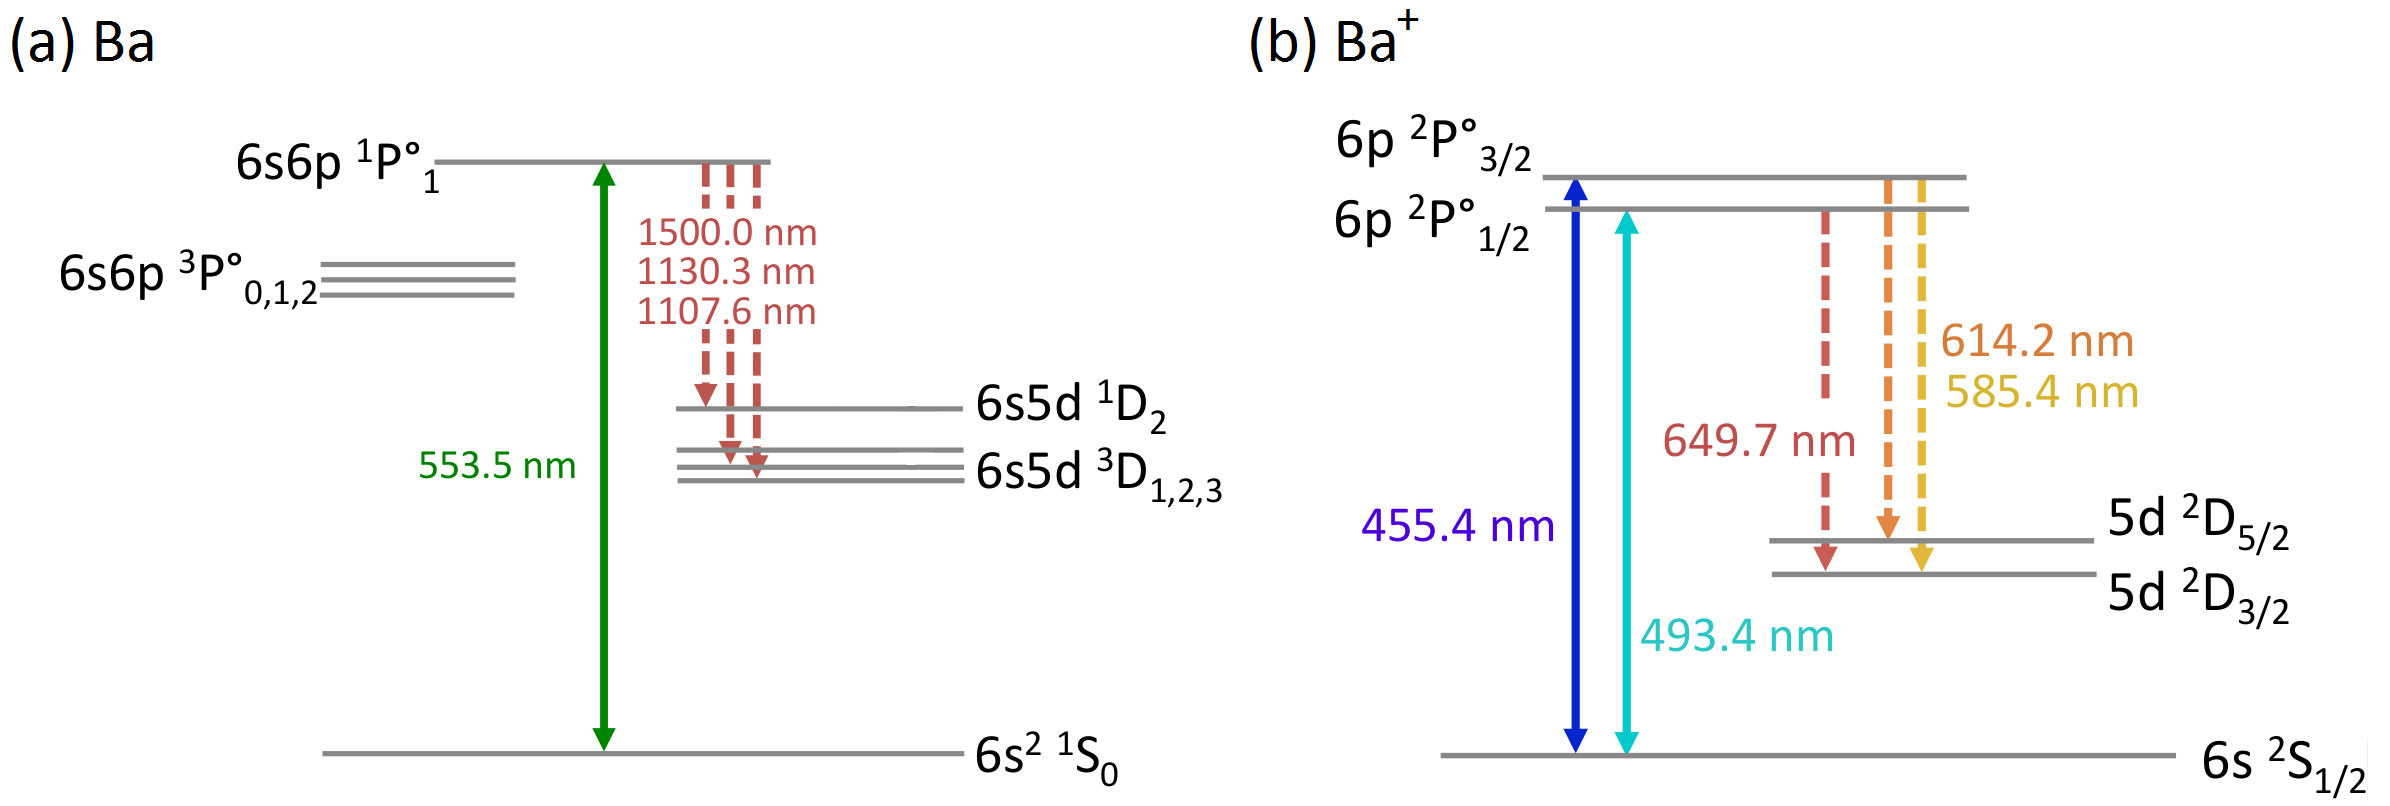
\includegraphics[width=.9\textwidth]{figures/elevs.png}
	\caption{Energy level diagrams for (a) Ba and (b) Ba\textsuperscript{+}}
    \label{fig:elevs}
\end{figure}

These energy levels and their transition rates are well known, and are documented in the NIST tables [ref].  Single atom/ion detection by spectroscopy generally requires lasers to provide transitions out of the metastable D states once the atom/ion decays into one of them, in addition to the main excitation laser.  For the atom, this requires three additional infrared lasers, and single atom trapping/detection in a magneto-optical trap (MOT) is achieved in [ref Ba MOT].  Single Ba\textsuperscript{+} observation requires only two lasers if the $^{2}$P$_{1/2}$ excited state is used.  This is demonstrated in [ref something that does this ... is there something?  How about the Carleton group?].

\section{Matrix Isolation Spectroscopy}

The spectroscopy of a species trapped in an inert solid matrix is called matrix isolation spectroscopy, the concept of which was pioneered around 19?? by [that one guy] [ref ... maybe [1] of ba spec].  Though absorption and emission are significantly broadened and shifted, a species can retain similarities to its vacuum counterpart, such as quantum numbers.

Studies of some matrix isolation systems have been made.  The most thoroughly studied has been Na(?) in solid matrices of (Ar, Kr, Xe ?)... (Na? Mg?)...[refs]

We are of course interested in the spectroscopy of Ba and/or Ba\textsuperscript{+} in SXe matrices, and this particular system has not been studied until recently.  The first report of the spectroscopy of neutral Ba in SXe, along with candidate fluorescence peaks for Ba\textsuperscript{+} in SXe, was published by our group in [ref ba spec], and conversations following this publication with ???'s group in ??? have confirmed our basic observations of the absorption spectrum of Ba in SXe.  

From here forward I will refer to the host species as Xe and the guest as Ba/Ba\textsuperscript{+}, specific to our system.  The leading interaction between {\color{gray}[put this here if the van der waals is only necessarily the force for Ba in particular]} the Ba/Ba\textsuperscript{+} and a neighboring Xe atom is a {\color{gray}(the)} Van Der Waals (sp?) force, an induced dipole-dipole interaction.  Xe is the most polarizable (sp?) of the noble gases.  

The forms for this force(?) is shown in Eqn. [ref van der ba] for Ba and Eqn. [ref van der ba+] for Ba\textsuperscript{+}.  {\color{gray}Talk about it.}

This binding between the Ba/Ba\textsuperscript{+} and its surrounding Xe atoms results in vibrational modes, and the Franck Condon (sp?) principle applies.  Fig. [ref fig franckcondon] helps illustrate this effect.  In a cold matrix, the system will be in the ground vibrational state before excitation.  The distribution of the wavefunction, even for the ground state alone, overlaps in space in general with more than one of the excited state vibrational modes, resulting in a broadening in energy of the absorption.

Rapid decay occurs to the lowest vibrational mode in the excited state before electronic decay can occur [ref] {\color{red}[is this just for Ba?]}.  Then a similar broadening in emission energy occurs as several overlapping vibrational mode wavefunctions exist in the ground electronic state, and a redshift is also observed as some energy was dissipated into phonons in the crystal in vibrational mode decays.  {\color{blue}\textbf{(How can you get a blueshift?)}}

Shifts and broadening in absorption and emission depend in general on the distribution of Xe atoms around the Ba/Ba\textsuperscript{+}.  The fcc crystal structure of the Xe restricts these environments to discrete number of so-called matrix sites, defined by (a) whether the Ba/Ba\textsuperscript{+} is {\color{red}[intersituational or whatever -- is that still a thing?]}, and (b) the number of vacancies in the Xe matrix surrounding the Ba/Ba\textsuperscript{+}.  Experimental observation of emission peaks from different matrix sites of [Na] in solid noble gases is reported in [ref(s)], with theoretical calculations in [ref(s)] attributing observed peaks to specific vacancy distributions defining the matrix sites (maybe this has been done?).

Energy level transition probabilities can also be affected in a matrix.  Distortions in electron wavefunction shapes by asymmetric matrix sites can affect radiative transitions by altering parity [ref].  If electronic potential energy curves cross each other, nonradiative transitions can also become allowed for otherwise forbidden transitions [ref].  {\color{red}(Is a phonon emission called a nonradiative transition / does this actually happen?)}

\emph{Jahn-Teller?}

The detectability of a single atom/ion can depend greatly on altered transition rates.  For example, in the Ba atom, matrix-allowed decay of the $^{1}$P$_{1}$ to the $^{3}$P states could be much stronger than the main transition back to ground, which would suppress fluorescence and make single-atom detection impossible.  But the matrix could also help by strengthening decays from the D states back to ground, eliminating any need for re-pump lasers to keep the transition cycle going.  